
\chapter{A Global Address Space}\label{ch:global}

\begin{chabstract}
    This chapter will describe the method by which Twizzler manages a global namespace, starting with how we define
    memory objects, how we name data within the space, and how we avoid coordination when assigning object IDs. We will
    then discuss object ID collision, and the probabilistic arguments therein. Finally, we will discuss two
    implementation details about how we provide software and hardware access to data in the global address space on
    current hardware.
\end{chabstract}

Constructing a global address space of all data means that any piece of data must be, in principle\sidenote{The ability
    to name a piece of data is disconnected from the \emph{rights} to access that data. Furthermore, \emph{discovery} of a
    name can also limit an application's ability to name data in practice, even if in theory it can name any data in the
    address space. These topics will be discussed further in Section~\ref{sec:sec}.}, namable from any
context. As such, any identification of data will need fairly long names if it is to contain all data within a (possibly
large) system. It is important to note here that I am using the term ``name'' to refer some an authoritative naming
system within which each piece of data has a single, unique name. I am not talking about, for example, C strings or a
path. In addition to naming data, a global address space will need a mechanism to ensure that names are in fact unique.

\section{Memory Objects}
To address these problems, \Twizzler organizes data into \emph{objects}. Each object is
identified by a unique 128~bit \emph{object ID}.
Objects provide contiguous regions of memory that organize
semantically related data with similar lifetime and permissions.
Applications access objects via
mapping services (discussed later in this chapter) by mapping each object into a contiguous range
in the address space, though the address space itself may be densely or sparsely mapped.
Objects can be anywhere from 4~KiB (the size of a page) to 1~GiB; the upper bound on object size is
an implementation choice, and not fundamental to the design.

%TODO maybe move this elsewhere
%\Twizzler uses objects as the unit of access control, building off a
%read/write/execute permissions model which mirrors that of memory management units in modern
% processors. This is a direct consequence of avoiding the kernel for
%persistent data access---it can set policy by programming the MMU, but must leave enforcement up to
%the hardware which, in-turn, defines what protections are possible.

%(it arises because of our persistent
%pointer design, discussed later).
An object, from the programmer's perspective, is flexible in its
contents---for example, it could contain anywhere from a single B-tree node to the entire B-tree.
Often, an object would contain the entire tree, since the entire tree is typically subject to
the same access semantics by programs, and there are overheads associated with objects that can be
amortized over larger spaces. Data and data structures that are too large for one object or require
different access permissions can span multiple objects with references between them.

Via objects, we gain a mechanism to name data. Since objects have a maximum size, we can simply index into them at a
byte level and form a name of a piece of data within object $X$ as a tuple of $(X, n)$ for an $n$ byte offset into the
object. If all object IDs are unique (which we will discuss later in this chapter), then the tuple fits our requirement
for an authoritative name.

One might question the decision to name data via a byte offset instead of a richer set of semantics. Our reasoning is
based around the level of the system we are currently working with. The basic construction of a global address space
with fixed-size object IDs and offsets is designed to be an \emph{underlying component} of a richer, higher level API.
Indeed, even our notion of invariant references that we will discuss in the next chapter is a ``low level'' mechanism.
Nothing prevents higher-level APIs and models from being built atop our lower level models---in fact, we plan for that!
The low level address space consruction is designed to be useable across a variety of languages and environments, not to
mention its intended use by hardware devices.

\paragraph{Objects Express Locality}
The primary reason that Twizzler organizes the global address space into objects instead of simply providing a large,
192~bit address space for all data is that it is useful to chunk the address space. We will see one major application of
chunking in the next chapter (invariant pointers), but there are several other reasons we use objects. First, allowing
the kernel to operate on objects instead of byte ranges dramatically simplifies the implementation and allows APIs and
services to operate on whole objects at a time. One can think of this as the same underlying reason that virtual memory
mappings operate on pages and not on bytes.

Another major purpose of objects is in allowing the programmer to use a direct, logical expression of locality.
The ability to group data as either semantically related, access-rights-equivalent, or as ``likely to be used at the
same time'' is fundamental to systems design. Programmers often group data for performance reasons like improving cache
hit rate, or choose explicitly to \emph{separate} items to avoid false sharing. Providing a logical expression of
locality through objects enables these kinds of design that programmers often do.
\begin{SCfigure}
    \centering
    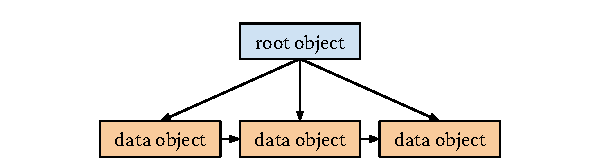
\includegraphics[width=\linewidth]{fig/objectchain1.pdf}
    \caption{Using a root object as an index to list multiple data objects that can be viewed logically as a contiguous block of data.}
    \label{fig:objchain1}
\end{SCfigure}

\begin{SCfigure}
    \centering
    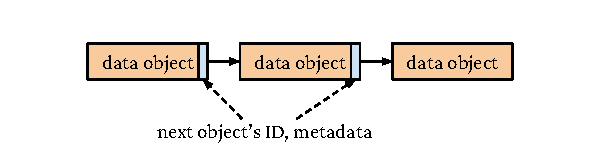
\includegraphics[width=\linewidth]{fig/objectchain2.pdf}
    \caption{Similar goals as in Figure~\ref{fig:objchain1}, but here we do away with the index object.}
    \label{fig:objchain2}
\end{SCfigure}
\paragraph{Chaining Objects}
The 1~GiB maximum object size may seem quite limited, but this may be because it is natural to think that they are
Twizzler's analogue to files in \unix. This is not the case---they are more similar to pages. If one wanted a
file abstraction in Twizzler, wherein the size of the file can grow largely without bound, we can simply chain multiple
objects together. Figures~\ref{fig:objchain1} and~\ref{fig:objchain2} show some possible schemes for accomplishing such
chaining, wherein we either form a linked list of objects (which would be effective for small, linear-accessed objects)
or have an index object that provides a list of data object for this ``file''. A variety of mechanisms are possible,
ranging from those depicted here, to nesting such solutions and forming an ``indirect block'' style of tracking data.
Since the minimum object's \emph{physical} size is 4~KiB, the overhead of having extra indexing objects is low.



\section{Object IDs}

We already discussed above that object IDs are 128~bits in size, but we should take a moment to discuss this choice,
along with how IDs are allocated. One aspect of our global address space I haven't touched on is coordination on IDs---that is,
when creating a new object, we must assign it an ID. Where does that ID come from?

One solution is via a centralized mechanism---some server hands out IDs when asked. The trouble here is scalability:
that centralized server will be quickly overloaded. Furthermore, the stated aim of our system is to allow devices and
nodes to act more independently to enable more concurrency. Yet a centralized solution would force them all through this
single bottleneck. Another similar solution would be a federated ID system, where we allocate ranges of IDs to a set of
centralized allocators, similar to MAC addresses. While a federated approach alleviates the problem somewhat, it still
has scalability problems and requires some out of band coordination ahead of time.

Part of the reason we selected a large ID space in the first place is to make it possible to assign IDs without
\emph{any} coordination. To ensure object ID uniqueness, we assign IDs by randomness. As long as we can ensure a high
enough chance of avoiding collision in the ID space, this method is scalable and fast.

We employ a probabilistic argument for avoiding collisions in the
object ID space. Since object IDs are generated randomly, we can model object IDs as an occupancy
problem in a space of $N = 2^{128}$ bins. Thus the probability of collision
is~\cite{motwani95}:

% TODO center equations
\begin{gather*}
    1 - e^{-
            \eqnmarkbox[NavyBlue]{m1}{m}
            (
            \eqnmarkbox[NavyBlue]{m2}{m}
            -1) / 2
            \eqnmarkbox[Orange]{n}{N}
        }
\end{gather*}
\annotatetwo[yshift=0.5em]{above}{m1}{m2}{\# of objects}
\annotate[yshift=-0.2em]{below}{n}{\# of object IDs}

If a system were to create millions of objects per second over the course of hundreds of years, the
probability of ID space collision is approximately 1 in $10^{-7}$. However, such a system is all but
guaranteed to suffer hardware errors that flip bits\sidenote{Take DRAM bit error from cosmic rays,
    for example.} in that time frame, and so an ID space collision is dramatically more likely to be
sourced from a hardware malfunction\sidenote{This is a common comparison when considering
    probability of a randomized computer process~\cite{hollingsworth:ssr97}.}. Further, the ID space
could be expanded to 256~bits, which would dramatically reduce the collision chances.

The reliance on randomized ID allocation is the primary reason we chose to make our object ID space
so much larger than some previous approaches~\cite{pmdk,pmdk-pointers}. Consider that if $N = 2^{64}$
bins, the probability of collision with just one billion objects is around 2\%. Increasing $m$ to
one object per person brings the collision probability up to nearly 75\%. Of course such an ID space
is usable if the ID are allocated via coordination with a centralized allocator, but if
we wish to allow object ID creation at scale, avoiding coordination is vital\sidenote{As we will
    discuss in the next chapter, some of these previous approches chose to put up with coordination and
    centralization because of the way they encoded their references. Twizzler uses a different method
    that allows ID space to be much larger.}. These alternative approaches with smaller ID spaces lead to problems when
sharing, since moving an object from one node to another requires either coordination or application-specific fixup
operations to avoid collisions.

\section{Mapping Back to Virtual Memory}



While virtual addresses are the wrong abstraction
for data access in a data-centric system, modern hardware provides (and often requires) the use of virtual address
hardware that we can leverage for protection and isolation, adding additional ephemeral state. Often these virtual
address spaces are the only method for applications to access memory. Thus Twizzler uses virtual memory hardware to
provide a data object access mechanism to programs.

\Twizzler defines objects called ``views'', which (among other things, see Chapter~\ref{ch:twizzler}) define the current
layout of the virtual address space. Twizzler
provides access to data objects by mapping them into the virtual address space
behind-the-scenes (via \libcore). The view object contains structures to define the layout of the
virtual address space which the kernel reads and uses to program the MMU accordingly.

Figure~\ref{fig:view} shows how view objects lay out the address space of any threads running inside
that particular view. View objects are manipulated by userspace and interpreted by the kernel. When
applications map objects, they update the view to specify that that object should be addressable at
a specific location. On a page-fault, the kernel reads the view and maps the object at the requested
location. The view object is laid out like a page-table, where each entry in the table corresponds
to a slot in the virtual address space. Each table entry contains an object ID and requested
protection bits to further protect objects atop access control mechanisms (similar to
\texttt{PROT\_*} in \texttt{mmap}).

\begin{SCfigure}
    \centering
    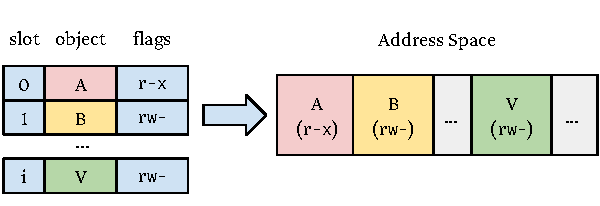
\includegraphics[width=\linewidth]{fig/view}
    \caption{Layout of a view object. The kernel consults the view object's mapping on page-fault,
        and maps in the requested objects at the appropriate location in the virtual address space.}
    \label{fig:view}
\end{SCfigure}

When a page-fault occurs, the fault handler tries to handle the fault by either doing copy-on-write,
checking permissions, or by trying to map an object into a slot if the view object requested one.
If it cannot handle the fault (due to a protection error or an empty entry in the view
object), it elevates the fault to userspace where \libcore handles it, possibly by killing the
thread, or possibly by mapping an object if the slot is ``on-demand''. This is similar to userspace
paging systems~\cite{l4,accetta:usenix86s}. When the kernel
maps an object into a slot, it updates the address space's page-tables appropriately.

Note that the use of virtual memory hardware and temporary object mapping into an ephemeral space does not mean that we
aren't using a global address space. In fact, in the next section we'll discuss \emph{another} non-global address space
that we make use of. Instead, think of these address spaces as implementation quirks for specific hardware. On x86, the
use of virtual addressing is all but required---if we had other hardware and addressing designs, we would have a
different layer here for providing actual object access. Finally, applications can ignore most of the \libcore mapping
stuff, since they still talk about data via the object ID and offset tuple.

\section{A Logical Address Space}

The interface presented to hardware must enable interaction with a
\textit{heterogeneous memory system} and support the abstraction of an object space rather than a
collection of flat memory spaces. Unlike applications, hardware has no need for
a global address space. Rather, hardware must
have the ability to transfer large chunks of objects to, from, and around memory, access memory words, and must be able to
handle access to different \emph{types} of memory, preferably in a way that is largely transparent to
applications.

It's important to note that here when I am talking about \emph{hardware}, I am drawing an important distinction between
the software (or firmware) running on a hardware device, and the hardware itself. The former am I grouping in with
software in general, as in the limit, we want that software (or firmware) to interact with data and other applications
just as any other piece of software might. By contrast, the hardware is the substrate upon which the software runs.
Hence while software sees and interacts with a global address space, the hardware sees but wires coming out to
electrically interact with other components.


Both software and hardware must have a way of translating a
name for some piece of data into a physical address. The software's method is to rely on mapping functionality provided
by the hardware, thus kicking the can down the road. The hardware must therefore know how to translate an object ID and
offset into physical memory.
This mapping may change frequently as the OS changes allocation of physical
pages to data (\eg, to persist a piece of data).
Hardware need only know
the mappings for a short time, and need not even care about the ``canonical''
name for the object or piece of data---it simply needs to know
how to access data in memory
for a single operation. In contrast, software must have longer-term mappings, and must
be able to support data shared between threads, potentially mapped into the threads
in different places.
Our design must support appropriate abstractions for both software and hardware,
allowing software to name data while providing hardware and
the operating system with the ability to move that data in, out of, and around physical memory, preferably with
compatibility for
existing hardware functionality.

We use an additional abstraction that sits underneath the global address space---a \emph{logical address space}. The
logical address spaces allows hardware to address data without needing knowledge of the data's physical location. Today,
hardware must worry about emitting loads and stores to physical memory, but in a world of heterogeneous physical memory,
the location of data is likely to change overtime. Ideally, this movement will be transparent to software (with the
exception of setting policy), but for hardware, it cannot be. Requiring hardware to access a global object space through a $\langle \mathit{object},
    \mathit{offset} \rangle$ tuple is unnecessary overhead and complexity---hardware need only ever
access the ``working set'' of objects currently undergoing computation. Thus, the logical address space
maps objects within it to physical memory pages, managed by the
operating system. This solves the heterogeneity problem by allowing hardware to refer to data within
objects instead of physical addresses, whose lifetimes are much smaller than the objects, and
doesn't require hardware to emit (likely large) addresses for the global address space.

\begin{SCfigure}
    \centering
    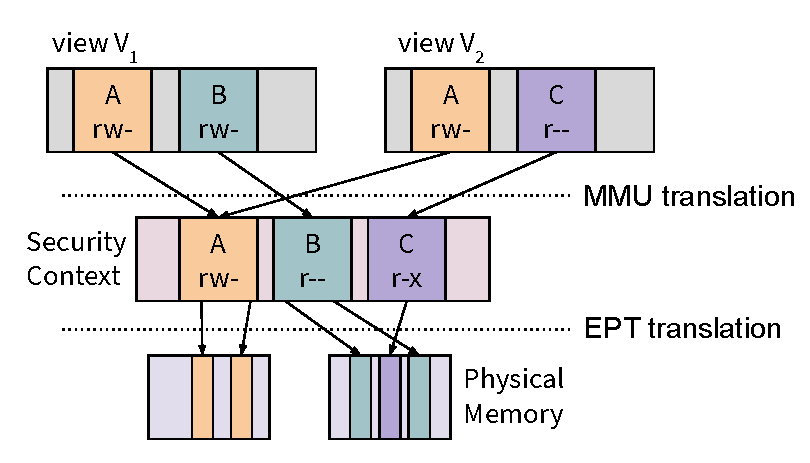
\includegraphics[width=\linewidth]{fig/2level}
    \caption{Two-level translation scheme. The top level maps objects in virtual memory (defined by view
        objects) to those in object-logical space. The layout of the second level address space is managed
        by the kernel, since it is not user-facing, and the permissions are derived from a security context
        object. The second level maps to physical memory.}
    \label{fig:twolevel}
\end{SCfigure}


While SASOSes are not a viable solution to the problem of persistent pointers, they are
\emph{a} solution to implementing the logical object space.  Hardware, and the CPU, are
directly connected, reducing the cost of invalidation and coordination of an address space.
Additionally, this address space is \emph{intermediate} and hidden from programs---a virtual
address is translated to the logical object space, after which the address is translated to a
physical location (shown in Figure~\ref{fig:twolevel}) by a second address translation. The result is that all devices
(including the lower level parts of the CPU) can share a single map of current objects in the logical object space. We
implement this on current x86 hardware via a combination of the IOMMU and the Extended Page Tables, and will discuss
this in more detail and how we use it to enhance security and low level kernel implementation in Chapter~\ref{ch:twizzler}.

\begin{chconc}
    A global address space provides a way for us to organize all data, and giving all data an authoritative name via an
    object ID and an offset allows us to provide a substrate for building more complex semantics later. Importantly, the
    uniqueness of object IDs and the isolated process for generating them means that we can avoid coordination on
    organizing the global ID space. As we will see, the choices of a large ID space that needs little coordination will
    play a big part of our solution to distributed memory. But now we are left with a question: if we name data via a
    tuple of an object ID and an offset, how do we implement an actual pointer?
\end{chconc}